\newpage
\section{Theoretisch Grundlagen der Named Entity Pipeline} \label{infos}

\subsection{Text Preprocessing} \label{TextPreprocessing}
Text Mining bezeichnet den Prozess, um wesentliche bekannte aber auch unbekannte Informationen aus Textdaten zu
generieren~\footcite[\vglf][\pagef 1]{mohan.2015}
Die Verarbeitung von unstrukturierten Textdaten wird auch als \ac{KDT}
bezeichnet und spielt eine signifikate Rolle in Anwendungsgebieten wie

\begin{itemize}
    \item Information Retrieval
    \item Information Extraction
    \item Natural Language Processing~\footcite[\vglf][\pagef 1 f.]{mohan.2015}
\end{itemize}
Im Wesentlichen geht es in allen \og Anwendungsgebieten um die Wissen durch das Mining der Texte zu generieren.

\begin{figure}[H]
    \caption{Text Mining Prozess}\label{fig:2_1_1_KDT_Process}
    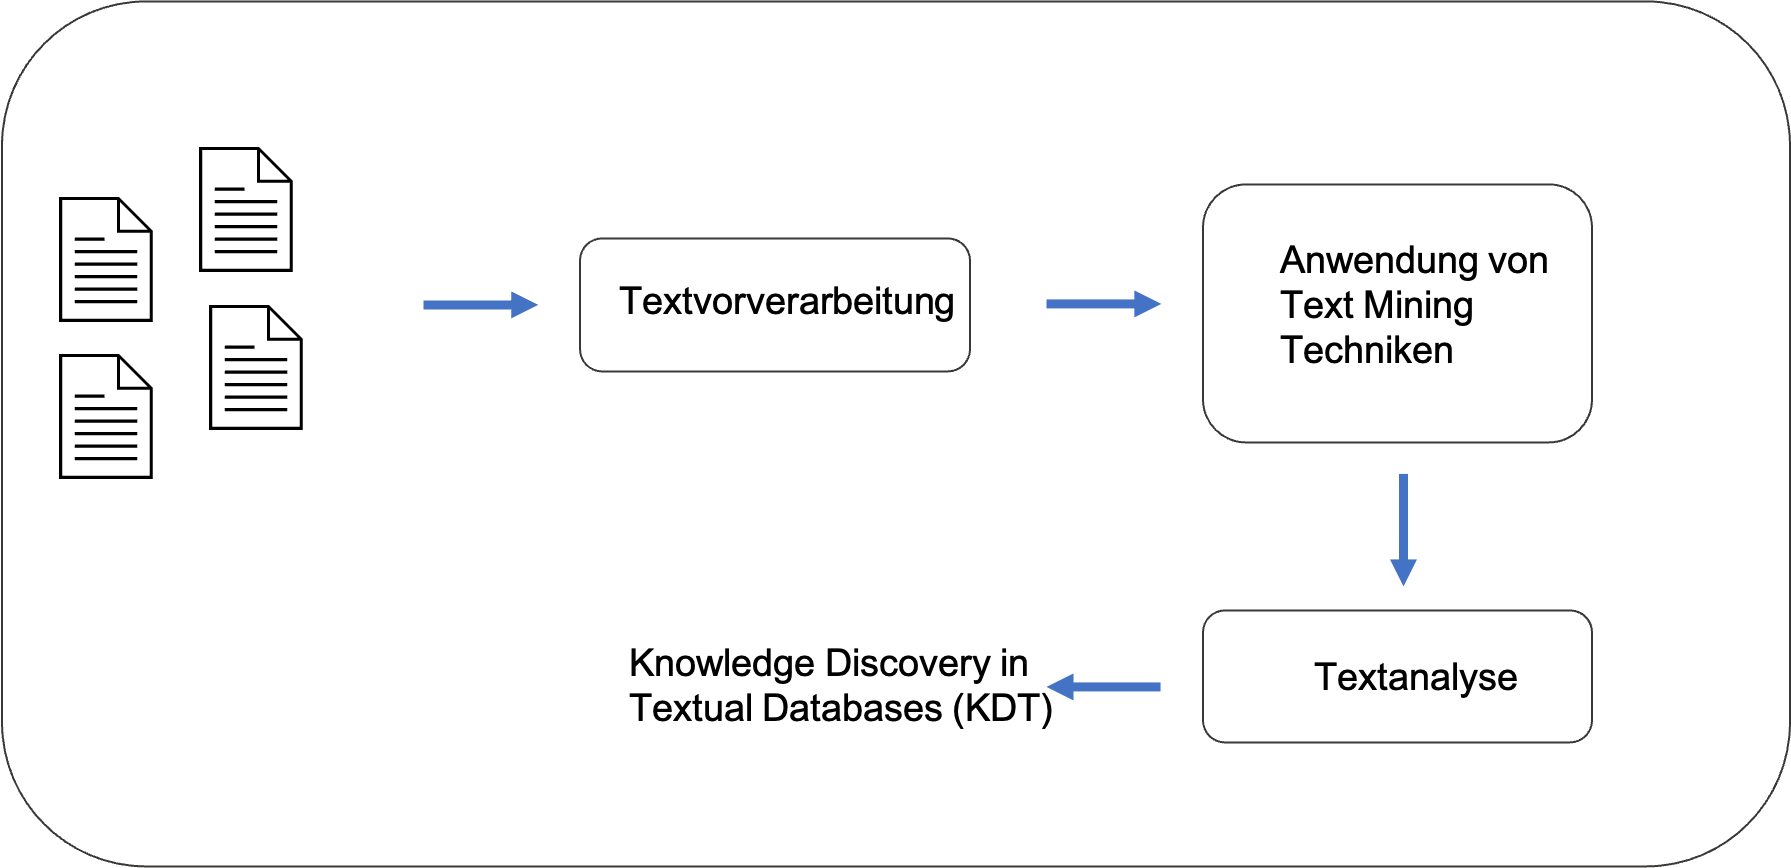
\includegraphics[width=0.9\textwidth]{2_1_1_KDT_Process}
    \\
    \textit{Quelle: Eigene Darstellung in Anlehnung an}~\cite[\pagef 1]{mohan.2015}
\end{figure}

Wie der Abbildung~\ref{fig:2_1_1_KDT_Process} entnommen werden kann, stellt die Vorverarbeitung von Volltextdaten bei nahe
zu jeder Aufgabe im \ac{NLP} einen essentiellen und kritischen Schritt dar,
da hierbei die fundamentale Basis für die Weiterverarbeitung
sowie die Entwicklung der Modelle geschaffen wird.~\footcite[\vglf][\pagef 2]{gurusamy.2014}
Der Begriff der Textvorverarbeitung umfasst dabei die Anwendung unterschiedlicher Techniken/Methoden, bei
denen die Textdokumente für die eigentlichen Zielsetzungen vorbereitet werden.
Gängige Techniken für die Vorbereitung der Texte für die nachgelagerten Analysen können folgendermaßen aufgeteilt
werden:~\footcite[\vglf][\pagef 1]{pahwa.2018}

\begin{itemize}
    \item Inhalte Extrahieren und Bereinigen
    \item Annotationen
    \item Normalisieren
\end{itemize}

Zu Beginn der Volltextanalysen stehen häufig die Rohfassungen der Texte zur Verfügung.
Diese gilt es im ersten Schritt technisch einzulesen.
Hierbei werden auch Daten mit eingelesen, dessen Informationsgehalt gering ist.
Beispielshaft zu nennen sind hier HTML tags, Werbung, etc beim Auslesen einer Website~\footcite[\vglf][\pagef 1]
{pahwa.2018} oder Grafiken, ASCII-Codes in PDF-Dateien.
Demnach ist das Ziel bei dem \textbf{Extrahieren und Bereinigen
der Inhalte} die Rohdaten soweit zu säubern, bis sich schließlich die reinen Texte als Resultat ergeben.
Nachdem die Texte um die technischen Störfaktoren bereinigt wurden, ist die \textbf{Tokenization} eine typische Technik
der Textextraktion.
In dem Prozess der Tokenisation wird der gesamte zu analysierende Text in einzelne Wörter, Phrasen,
Symbole, etc.
geteilt.
Hierbei wird das Ziel verfolgt die Bedeutung einzelner Wörter innerhalb eines Satzes zu analysieren.
Die Tokens dienen nämlich als Eingabewerte für viele weitergehende Prozessschritte.~\footcite[\vglf][\pagef 2]
{gurusamy.2014}
In jedem Text befinden sich Wörter, die wenig Informationsgehalt bei der Textanalyse bieten.
Solche Wörter werden auch als \textbf{Stop Words} bezeichnet.
Beispiele für solche Stop Words sind Artikel oder
Präpositionen wie \glqq{der}\grqq, \glqq{die}\grqq, \glqq{das}\grqq, \glqq{ein}\grqq,
\glqq{in}\grqq, \glqq{mit}\grqq, etc.
Im Analyseprozess stellt jedes unterschiedliche Wort eine eigene Dimension dar.
Durch die Entfernung der Stop Words wird somit die Dimensionshöhe reduziert bei gleichzeitiger Beibehaltung des
Informationsgehaltes des jeweiligen Satzes/Textes.~\footcite[\vglf][\pagef 3]{mohan.2015}\\
Neben der klassischen Methode, die Stop Words auf Basis einer vordefinierten Liste zu entfernen, sind diverse
mathematische und nicht-mathematische Methoden entwickelt worden, um Stop Words in Texten zu identifizieren und zu
bereinigen.\footnote{Detailiertere Informationen zu unterschiedlichen Methoden für die Entfernung von Stop Words
können{}\cite{mohan.2015} entnommen werden.}\\

Die Annotationen eines Textes sollen die Funktion des jeweiligen Wortes im Kontext des gesamten Satzes identifizieren.
Eine gängige Methode ist dabei das so genannte \ac{POS}-Tagging.
Jener ist ein Prozess, der die Zuweisungen einzelner Wörter zur \ac{POS} bzw{.} zu lexikalischen Klassenmarkern wie
Nomen, Verben, Adjektiven, usw{.} vornimmt.~\footcite[\vglf][\pagef 1]{kumawat.2015}
Bei der Erkennung der Funktion eines Satzes treten folgende Hauptprobleme auf:
\begin{itemize}
    \item Mehrdeutige Wörter
    \item Unbekannte Wörter
\end{itemize}
Ersteres stellt das wichtigste Problem dar.
Es gibt Wörter, für die es mehr als einen Tag geben kann.
Dieses Problem wird durch einen Fokus des Wortes im Satzkontext gelöst.~\footcite[\vglf][\pagef 1]{gurleenkaursidhu.2013}
Andersrum existieren Wörter, die zwar denselben Tag haben, jedoch unterschiedliche Bedeutungen im Satzkontext einnehmen.
~\footcite[\vglf][\pagef 1]{gurleenkaursidhu.2013} Eine Lösung ist hierbei die Betrachtung des einzelnen Wortes, statt dem
Kontext.
Das menschliche Auge kann solch eine Differenzierung schnell vornehmen, während es für eine Maschine mühselige Arbeit
und einen Lernprozess darstellt.
Wie zuvor angeführt, ist es für die automatische \ac{POS}-Erkennung notwendig ein Modell zu trainieren.
Hier wurden mit der Zeit diverse Methodiken entwickelt, die sich auf oberster Ebene in überwachte und unüberwachte
Methoden aufteilen.
Bei den überwachten Ansätzen wird das \ac{POS}-Modell auf Basis eines Datensatzes trainiert, bei dem die \ac{POS}-Werte
bekannt sind, während das Modell bei den unüberwachten Ansätzen die \ac{POS}-Werte selbst induziert, da dem
Trainings-Datensatz keine bekannten Werte vorliegen.~\footnote{Eine detailierte Übersicht über vorhandene \ac{POS}-
Methoden sind in~\cite{kumawat.2015} zu finden.}



Bei dem \textbf{Normalisieren} von Texten wird das Ziel verfolgt ähnliche Wörter zu vereinheitlichen bzw.
diese auf einen Standard zu bringen.
Dieser Prozess soll vor allem die Dimensionen reduzieren, um die Berechnungen zu vereinfachen und gleichzeitig die
Effizienz durch die Standardiesierung der Wörter erhöhen.
\newline
Bei der Normalisierung von Wörtern wird häufig auf die Techniken des \textbf{Stemming} oder der \textbf{Lemmatization}
zurückgegriffen.
Das Stemming ist ein Prozess, der zugrundeliegende Wörter auf den Wortstamm herunterbricht.~\footcite[\vglf][\pagef 5]
{khyani.2021}
Dieser Wortstamm ist im Ergebnis häufig kein echtes Wort, sondern oftmals eine Buchstabenkombination bzw.
ein Präfix, den viele Wörter gemeinsam haben.~\footcite[\vglf][\pagef 5]{khyani.2021}
Es existiert eine Vielzahl an Stemming-Algorithmen, dessen Performance vom jeweiligen Einsatzbereich abhängt, sodass
noch kein Standard etabliert ist.\footnote{Eine ausführliche Analyse unterschiedlicher Stemming-Algorithmen kann{}
\cite{jivani.2011} entnommen werden.}
\newline
Die Idee bei der Lemmatization ist das so genannte \grqq{Lemma}\grqq{} oder auch die Vokabularform eines Wortes
zu identifizieren.~\footcite[\vglf][\pagef 7]{khyani.2021}
Der Prozess ist ähnlich dem des Stemmings, jedoch mit dem Unterschied im Ausgabewert.
Während beim Stemming der Ausgabewert der Wortstamm ist und oftmals kein echtes Wort,
ist der Ausgabewert bei der Lemmatization das Grundwort aus beispielsweise einem Wörterbuch.~\footcite[\vglf]
[\pagef 7]{khyani.2021}
Die Abbilung~\ref{fig:2_1_2_Stem_Lemma} verdeutlicht die Unterschiede der Lemmatization und des Stemmings anhand
des englischen Wortes \grqq{change}\grqq{} bzw.
dessen Abwandlungen.

\begin{figure}[H]
    \caption{Stemming vs. Lemmatization}\label{fig:2_1_2_Stem_Lemma}
    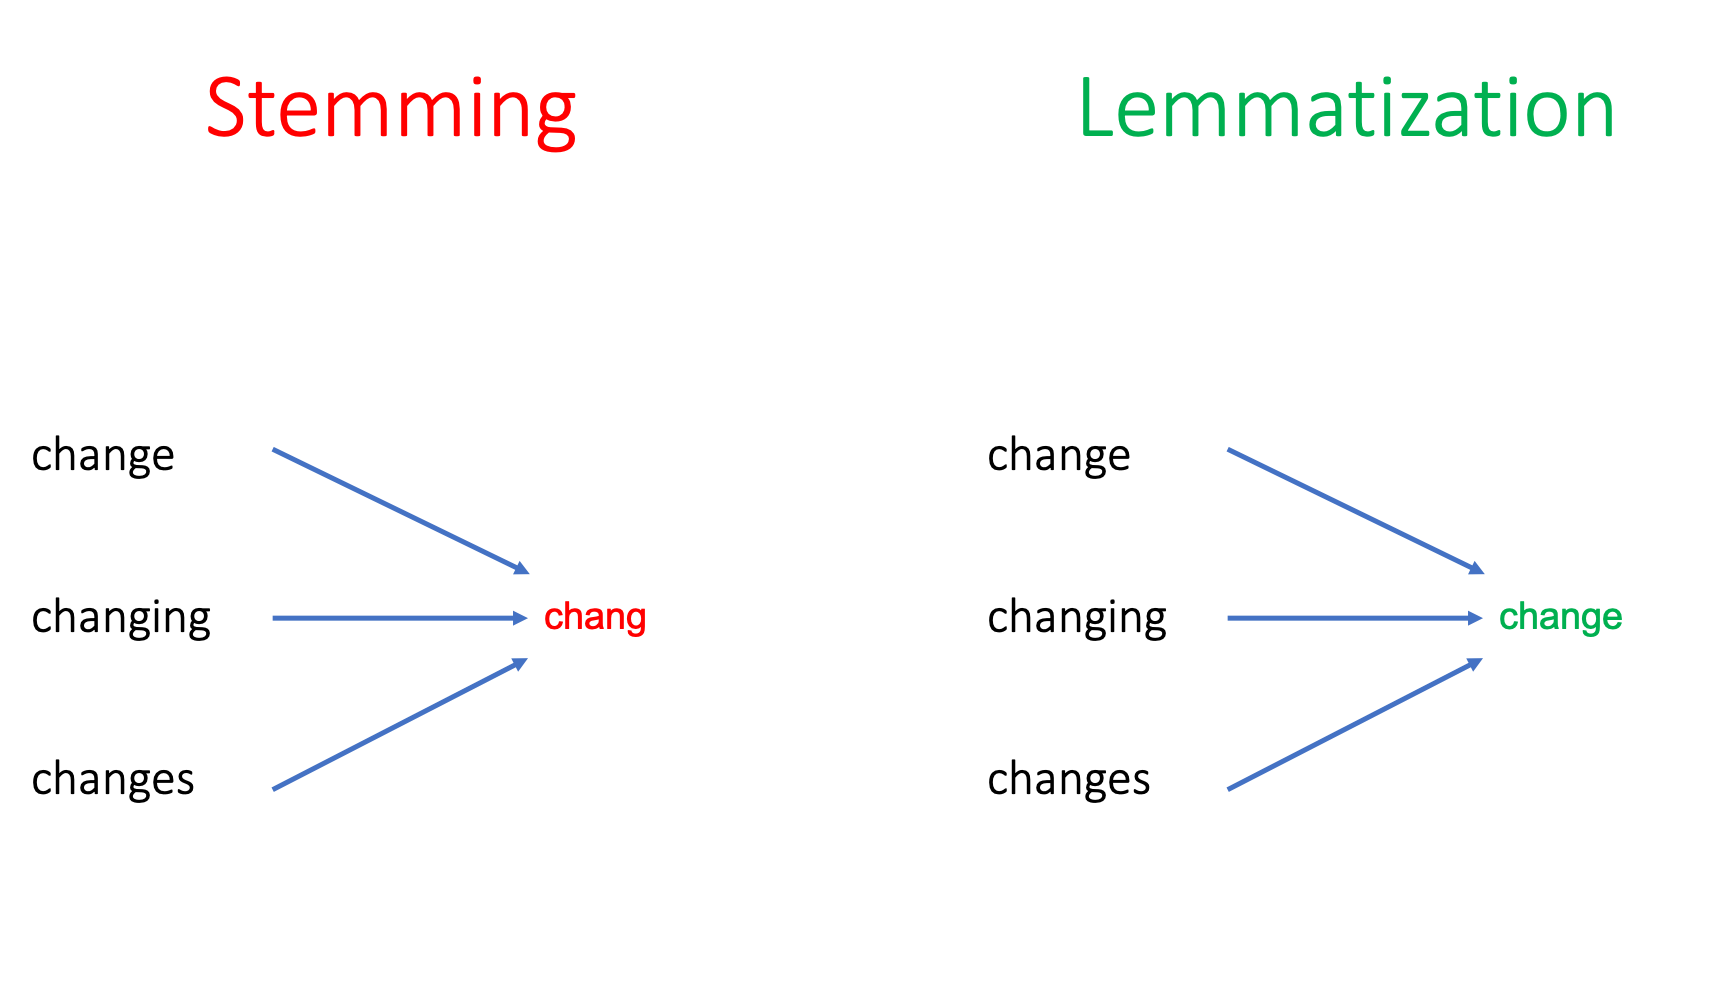
\includegraphics[width=0.9\textwidth]{2_1_2_Stem_Lemma}
    \\
    \textit{Quelle: Eigene Darstellung in Anlehnung an}~\cite[\pagef 7]{khyani.2021}
\end{figure}
Ein vorab durchgeführtes \ac{POS}-Tagging kann die Ergebnisse der Lemmatization optimieren.
Wenn das Wort \glqq{schloss}\grqq{} nämlich in einem Text als Nomen durch das \ac{POS}-Tagging erkannt wird,
dann handelt es sich dabei je nach Kontext entweder um ein Schloss zum verriegeln oder um ein Schloss als Gebäude.
Wird es dagegen als Verb identifiziert, so wird mit einer hohen Wahrscheinlichkeit zum Lemma \glqq{schließen}\qrqq{}
umgewandelt.

\subsection{Named Entity Recognition} \label{NER}

Mithilfe der \ac{NER} wird das Ziel verfolgt automatisiert Eigennamen in Texten zu identifizieren,
dessen semantische Typen wie beispielsweise Personen, Ort, Organisationen vordefiniert wurden.~\footcite[\vglf]
[\pagef 1]{nadeau.2007}
Die \ac{NER} kann nicht nur ausschließlich für die Extraktion von Informationen aus Texten genutzt werden, viel mehr
spielt sie eine wesentliche Rolle in einer Vielzahl von Anwendungen aus dem Gebiet des \ac{NLP} wie beispielsweise dem
Textverständnis, dem \ac{IR}, automatisierter Textzusammenfassungen und Übersetzungen, Fragenbeantwortungen, etc.
In der Forschung existiert eine Vielzahl an Definitionen für die zu erkennenden Eigennamen, die hauptsächlich in
folgende zwei Kategorien aufgeteilt werden können:
\begin{itemize}
    \item Generische (\zb Personen und Ort)
    \item Domänenspezifische (\zb Proteine, Enzyme und Gene)~\footcite[\vglf][\pagef 1]{li.2018}
\end{itemize}
Bei den in der \ac{NER} angewandten Techniken wird zwischen
\begin{itemize}
    \item Regelbasierte Ansätze
    \item Unüberwachte Ansätze
    \item Merkmalsbasierte überwachte Lernansätze
    \item Deep-Learning Ansätze
\end{itemize}
unterschieden, wobei die drei erstgenannten den traditionellen Ansätzen zugehörig sind.~\footcite[\vglf][\pagef 1]
{li.2018}
Regelbasierte Systeme beruhen auf manuell erstellten Regeln.
Die zugrundeliegenden Regeln können hierbei \zb aus domänenspezifischen Ortsverzeichnisen oder syntaktisch-lexikalischen
Mustern abgeleitet worden sein.\newline
Das Clustering ist ein typischer Ansatz für unüberwachte \ac{NER}-Systeme.~\footcite[\vglf][\pagef 6 f.]{nadeau.2007}
Auf Basis von Kontextähnlichkeiten werden geclusterte Gruppen generiert aus denen schiließlich die
Entitäten extrahiert werden.
Die Idee bei dieser Technik ist mithilfe eines großen Corpus lexikalische Muster und Statistiken zu berechnen, um daraus
auf im Text benannte Entitäten schließen zu können.~\footcite[\vglf][\pagef 4]{li.2018}\newline
Im Teilbereich der überwachten Ansätze ist \ac{NER} hauptsächlich eine Klassifikationsaufgabe.
Ausgehend von annotierten Datensätzen werden Merkmale entwickelt, um jedes Trainingsbeispiel zu repräsentieren.
~\footcite[\vglf][\pagef 4]{li.2018}
Für die Entwicklung der Modelle kommen dann Algorithmen des \ac{ML} zu Einsatz, um aus den gegeben annotierten
Datensätzen Vorhersagemodelle für noch ungesehene Daten zu erlernen.~\footcite[\vglf][\pagef 4]{li.2018}
Essentiell in überwachten \ac{NER}-Systemen ist die Entwicklung der Merkmale.
Merkmalsvektoren abstrahieren dabei den Text, bei der ein Wort durch einen oder mehrere boolische, numerische oder
nominale Werte dargestellt wird.~\footcite[\vglf][\pagef 7]{nadeau.2007}\newline
Neben den eben erläuterten traditionellen Methoden für die \ac{NER} wurden in den letzten Jahren Ansätze im Bereich des
\ac{DL} entwickelt, welche sich bewährt haben und Spitzenergebnisse erzielen.~\footcite[\vglf][\pagef 5]{li.2018}
Der Einsatz von \ac{DL} hat wesentliche Vorteile gegenüber den traditionellen Methoden.
Zum einen ist es durch die besondere Architektur und den Verarbeitungsmöglichkeiten im Bereich des \ac{DL} über
mehrschichtige künstliche neuronale Netze möglich nicht-lineare Zusammenhänge zu erkennen und zu lernen und zum anderen
erleichtern \ac{DL}-basierte Modelle durch ihre Automation und Selbstständigkeit beim Lernen die Arbeit.~\footcite
[\vglf][\pagef 5]{li.2018}\newline
\newline
Die \ac{NER} umfasst zwei Teilaufgaben: Typenidentifikation und Grenzerkennung
Die Bewertung eines entwickelten \ac{NER}-Systems wird in der Regel durch den Vergleich mit den mennschlich getätigten
Annotationen vorgenommen.
Der Vergleich kann entweder über eine exakte oder durch eine partielle Übereinstimmungsevaluation vorgnommen werden.
~\footcite[\vglf][\pagef 3 f.]{li.2018}
Bei der exakten Übereinstimmungsevaluation wird geprüft, ob das System sowohl den richtigen Typen als auch die Grenzen
korrekt identifiziert.~\footcite[\vglf][\pagef 3]{tjongkimsang.2003}
Bei der partiellen Übereinstimmungsevaluation genügt es, wenn, unabhängig von den Grenzen, eine korrekte Identifikation
des Typen vom System vorgenommen wird, solange es eine Überschneidung zwischen den ermittelten Grenzen und den wahren
Grenzen gibt.
Bewertungskennzahlen für die Qualität des \ac{NER}-Systems sind Precision, Recall und der F-Score.
Um diese zu ermitteln, wird vorab die Anzahl der \ac{FP}, \ac{FN} und \ac{TP} Zuordnungen ermittelt.
\begin{itemize}
    \item \ac{FP}: Eine Entität wurde vom System erkannt, welche in Wirklichkeit keine ist
    \item \ac{FN}: Eine Entität wurde nicht vom System erkannt, welche in Wirklichkeit jedoch eine darstellt
    \item \ac{TP}: Eine Entität wurde vom System korrekt erkannt
\end{itemize}

Die Precision stellt sich dar als
\begin{align}
    Precision {=} \frac{\ac{TP}}{(\ac{TP}+{\ac{FP}})}
\end{align}
und kann als Verhältnis von richtig erkannten Entitäten zur Gesamtheit an identifizierten Entitäten interpretiert werden.

Der Recall
\begin{flalign}
    Recall{} {=} {}\frac{\ac{TP}}{(\ac{TP}+{\ac{FN}})}
\end{flalign}
bezieht die richtig erkannten Entitäten auf die Gesamtheit aller möglich gewesenen Entitäten.

Der ausgeglichene F-Score vereint die Precision und den Recall zu einem harmonischen Mittel:
\begin{flalign}
    F-Score{} {=} {}2 \cdot \frac{Precision \cdot Recall}{Precision + Recall}
\end{flalign}


\subsection{Named Entity Linking} \label{NEL}